% =============================================================================
% main.tex -- Systematic literature review in the ICICIC single-column format
% Compile: pdflatex main.tex && pdflatex main.tex
% =============================================================================
\documentclass[12pt,a4paper]{article}
\usepackage{icicic}
\usepackage{multirow}
\usepackage{needspace}

\begin{document}

\papermeta
  {Accuracy and Efficiency of Large Language Models for Title and Abstract Screening in Systematic Reviews: A Systematic Literature Review}
  {Mohammed Haddad$^{1,*}$}
  {$^1$Faculty of Sciences and Techniques\\
   University Abdelmalek Essa\^adi, Tangier, Morocco\\
   $^*$Corresponding author: mohammed.haddad@etu.uae.ac.ma}
  {Report date: November 15, 2026}

\paperabstract{Title and abstract screening is the most labour-intensive step of a
systematic review, and large language models (LLMs) are increasingly proposed to automate it.
We conducted a systematic literature review, reported according to PRISMA 2020, of studies
published from 2020 onwards that evaluate LLMs for this task. OpenAlex, PubMed, arXiv and
Semantic Scholar were searched on November 15, 2026; the review was executed with an agentic
pipeline (dual independent screening, independent adjudication, retrieval-augmented extraction
with verified quotations and a critic loop) under a full audit trail. Of 123 records, 115
were screened (Cohen's $\kappa=0.77$ between screeners) and 14 studies were included: 12
primary evaluations and 2 prior reviews. Reported sensitivity of LLM screening ranged from
0.73 to 1.00 and specificity from 0.81 to 0.99, with workload reductions of 65--85\% and
screening of 1,000 abstracts in under one hour. All studies were judged at high risk of bias,
mainly for their reference standard, and heterogeneous metrics precluded meta-analysis. LLMs
are credible high-sensitivity first screeners, but certainty is low and human oversight remains
necessary.}

\paperkeywords{Large language models, Systematic review, Title and abstract screening,
Automation, Sensitivity and specificity, PRISMA 2020, Agentic AI, Evidence synthesis}

% =============================================================================
\section{Introduction}
Systematic reviews are the foundation of evidence-based practice, but they are slow: a
review registered in PROSPERO takes on average about 67 weeks from registration to
publication~\cite{borah}. Much of this effort goes into title and abstract screening, in which
two reviewers independently examine every retrieved record, often thousands of them, against
pre-specified eligibility criteria~\cite{cochrane}. The task is repetitive, error-prone, and
grows with the volume of the literature.

Large language models (LLMs) can read a title and an abstract, apply eligibility criteria
written in natural language and justify their decision, without the task-specific training
data that earlier machine-learning screening tools needed. A rapidly growing number of studies
have therefore evaluated general-purpose models such as GPT-4o, GPT-5, Claude, Gemini and
DeepSeek as screeners. Their results are scattered across clinical, preclinical, software
engineering and education domains, use different reference standards, and report different
metrics, which makes them hard to compare.

The objective of this review is to answer the question: \emph{how accurate and how efficient
are LLMs at title and abstract screening for systematic reviews?} Specifically, we summarise
(i) their sensitivity, specificity and overall accuracy against human reviewers, (ii) their
agreement with humans, (iii) the time and cost savings they deliver, and (iv) the factors
that make their performance vary. The review itself was produced with an agentic AI pipeline built on
LangGraph~\cite{langgraph}, described in Section~2 and in~\cite{repo}, so that every screening and extraction decision is
traceable.

% =============================================================================
\section{Methods}
The review is reported according to the PRISMA 2020 statement~\cite{prisma}. The protocol was
generated before any search and approved at a human-in-the-loop checkpoint; it was not
registered.

\subsection{Eligibility criteria}
Studies were included if they (I1) evaluated LLMs for title and abstract screening in
systematic reviews, (I2) reported sensitivity, specificity or overall accuracy, (I3) compared
the LLM with human or conventional screening, (I4) were published in English as journal
articles, conference papers or preprints, and (I5) appeared from 2020 onwards. Studies were
excluded if they (E1) did not use an LLM, (E2) addressed only full-text screening or data
extraction, (E3) reported no performance metric, or (E4, E5) fell outside the language and
time limits. Preprints were deliberately eligible, because this field moves faster than
journal publication.

\subsection{Information sources and search strategy}
OpenAlex, PubMed (E-utilities), arXiv and Semantic Scholar were searched on November 15, 2026,
through their public application programming interfaces. Three concept blocks were combined with
AND: \emph{large language models} (e.g., ``large language models'', ``LLMs'', ``pre-trained
language models''), \emph{systematic review screening} (e.g., ``title and abstract
screening'', ``study selection'', ``literature screening'') and \emph{performance} (e.g.,
accuracy, sensitivity, specificity). The blocks were compiled deterministically into
database-specific syntax: field-tagged \texttt{[tiab]} queries for PubMed, \texttt{all:} queries
for arXiv, and relevance-ranked keyword queries for OpenAlex and Semantic Scholar. The first
25 records per query were retrieved. All responses were cached so that the search can be
replayed exactly. Semantic Scholar refused the requests (HTTP 429, rate limit), so the
retrieved records come from the three other sources.

\subsection{Selection process}
Duplicates were removed by DOI and by fuzzy title matching (similarity $\geq 93$). Each record
was screened independently by two LLM reviewers (\texttt{qwen3:8b}, different sampling seeds,
temperatures and orders of presentation), which judged every criterion as \emph{yes},
\emph{no} or \emph{unclear} and justified their decision. Following standard practice, a
record was excluded only when it clearly violated a criterion. Agreement was measured with
Cohen's $\kappa$~\cite{cohen}. Disagreements were resolved by an adjudicator from a different
model family (\texttt{gpt-oss:20b}). Full texts were sought for the records with the highest
screening confidence (budget of 15). Open-access PDFs were parsed and indexed for hybrid
retrieval, combining dense embeddings, BM25 and reciprocal rank fusion~\cite{rrf}, with a
cross-encoder re-ranker~\cite{rag}. When no open-access full text existed, eligibility was
assessed on the abstract, and this is flagged.

\subsection{Data collection and data items}
For each included study an extraction agent filled a structured form from the re-ranked
passages: design, data set, LLM and method, comparator, outcomes, quantitative results,
main finding and limitations. Every value carries a verbatim quotation and its passage
identifier; quotations were automatically checked against the source text, and 92\% were found
verbatim. The outcomes were sensitivity (recall), specificity, accuracy or F1, agreement with
human reviewers, and time or cost.

\subsection{Risk of bias and certainty}
Risk of bias was judged in five domains adapted from QUADAS-2~\cite{quadas} to LLM evaluation
studies: dataset representativeness, reference standard, leakage, reporting of metrics and
reproducibility. The overall judgement is the worst domain. Certainty of each synthesised
finding was rated with a GRADE-inspired approach~\cite{grade}.

\subsection{Synthesis methods}
The protocol planned a meta-analysis. It was not feasible: the studies report different
metrics (sensitivity and specificity, recall and precision, F1, AUC or percent agreement)
against different reference standards. A structured narrative synthesis was therefore
performed, grouped into four themes. An independent critic agent checked every claim against
the evidence table; it requested two revisions and approved the third version.

% =============================================================================
\needspace{8\baselineskip}
\section{Results}

\subsection{Study selection}
The search identified 123 records (OpenAlex 75, PubMed 25, arXiv 23). After removing 8
duplicates, 115 records were screened. The two screeners agreed on 102 of them ($\kappa=0.77$,
substantial agreement~\cite{landis,mchugh}); the adjudicator resolved the remaining 13. In total, 74 records
were excluded and 41 passed screening. Of these, 15 reports were assessed for eligibility
(9 on the abstract only, as no open-access full text was available) and 26 were not sought
because of the budget cap. One report was excluded because it addressed full-text screening
only (E2). Fourteen studies were included (Figure~\ref{fig:prisma}).

\begin{figure}[!htb]
\centering
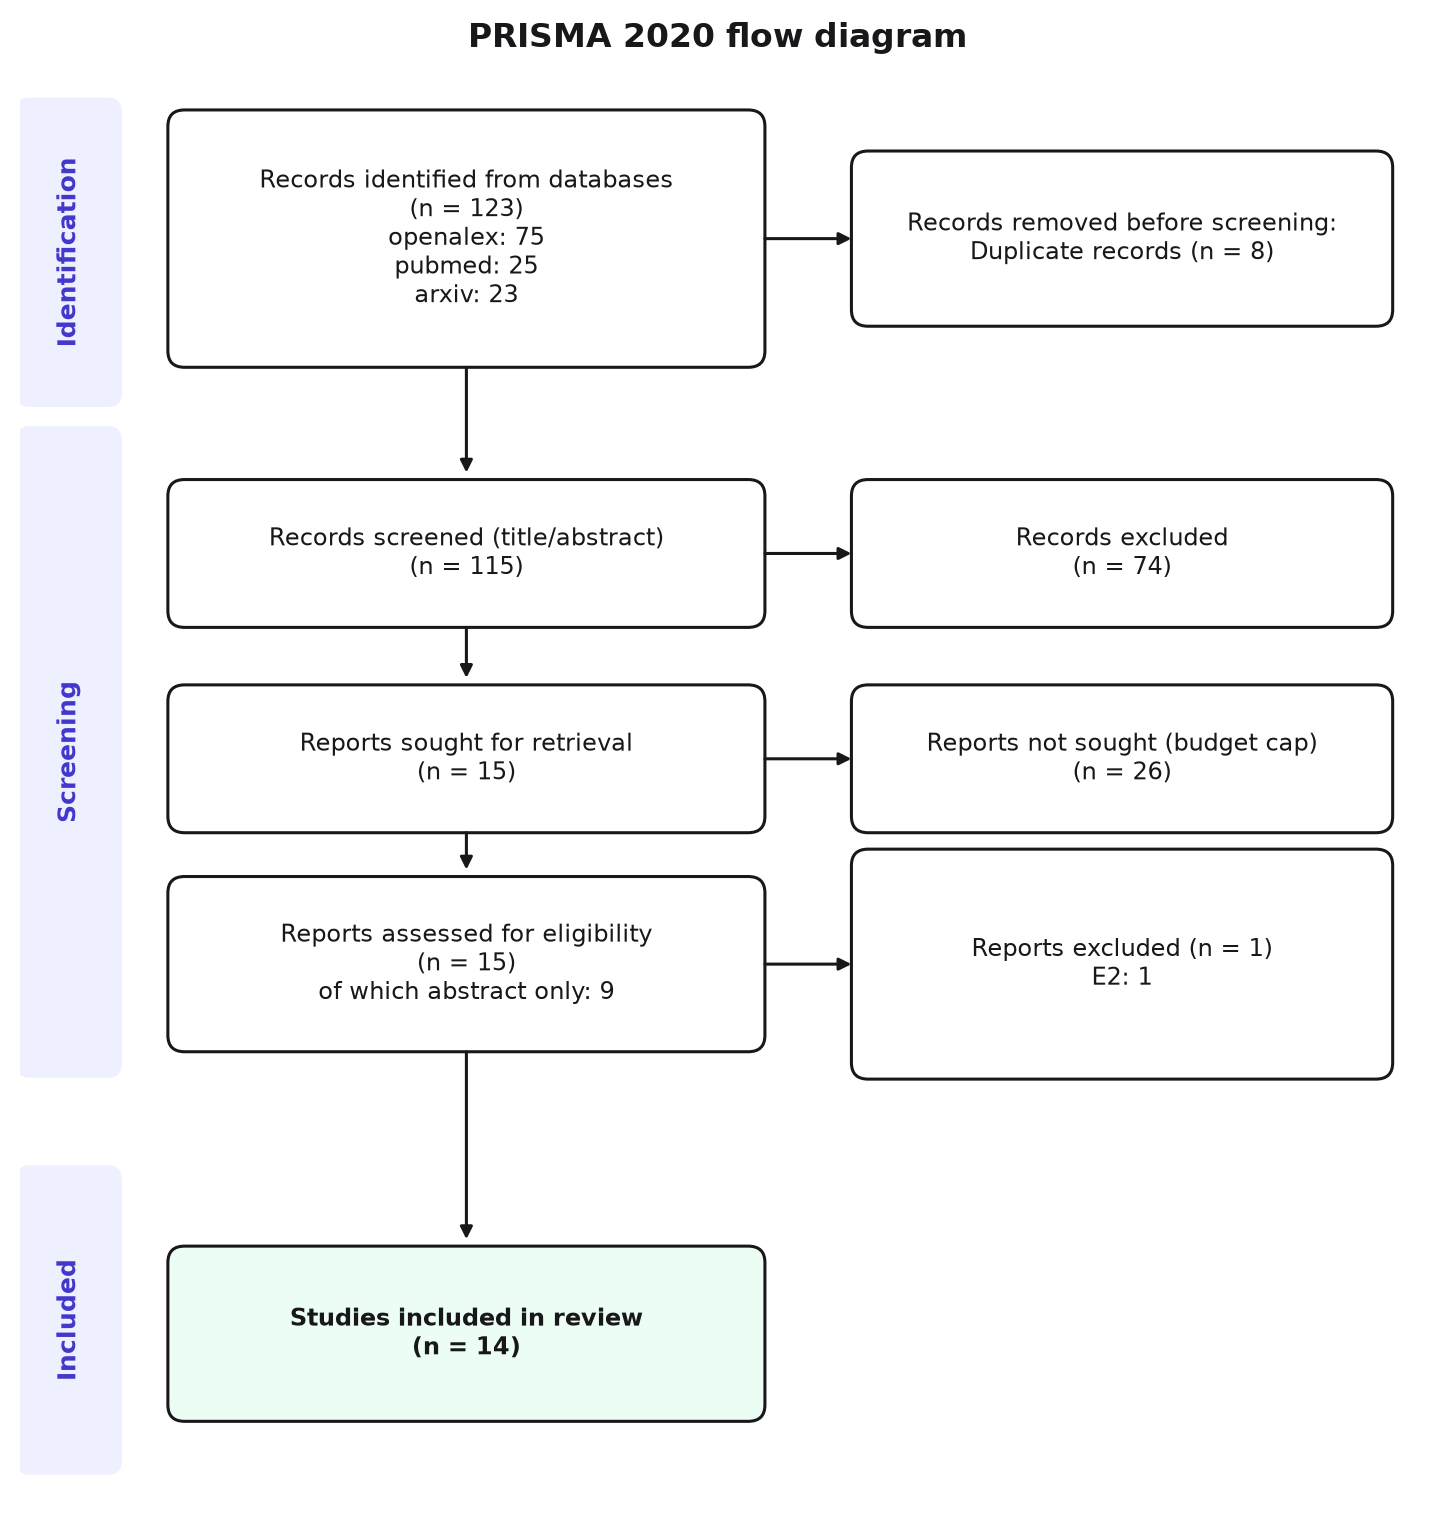
\includegraphics[width=0.66\linewidth]{prisma_flow.png}
\caption{PRISMA 2020 flow diagram of the study selection}\label{fig:prisma}
\end{figure}

\subsection{Study characteristics}
The 14 studies were published between 2025 and 2026 (Table~\ref{tab:char}). Twelve are primary
evaluations; two are themselves systematic reviews of LLMs in evidence synthesis~\cite{s014,s037}.
They are reported separately to avoid double counting. The primary studies covered clinical
medicine (thoracic surgery~\cite{s027}, orthopaedics~\cite{s038}, radiology~\cite{s035}, mental
health~\cite{s032}, health outcomes research~\cite{s008}), biomedical informatics~\cite{s002}, several
review types at once~\cite{s010,s031,s033}, and software engineering and education~\cite{s009,s036}.
The evaluated models were mostly proprietary (GPT-4o, GPT-4o mini, GPT-4.1, GPT-5, Claude 3.5,
Gemini 1.5/2.5) with some open models (DeepSeek R1, Llama 4). The usual reference standard
was the decisions of the original human reviewers.

\begin{table}[!htb]
\small
\setlength{\tabcolsep}{4pt}
\renewcommand{\arraystretch}{1.08}
\centering
\captionof{table}{Characteristics of the included studies}\label{tab:char}
\begin{tabular}{|p{2.5cm}|p{3.6cm}|p{3.6cm}|p{2.9cm}|}
\hline
Study & Data & LLM / approach & Comparator\\
\hline
Li 2026~\cite{s002} & 6,331 biomedical articles & DeepSeek R1 + rules + RAG, ensembles & manual screening\\
\hline
Fazeli 2026~\cite{s008} & 15,605 records, 5 SLRs & GPT-4o mini, custom prompt & expert reviewers\\
\hline
Hida 2026~\cite{s009} & 2 SE/education SLRs & 12 LLMs, 5 repeated runs & classical classifiers\\
\hline
Mosaed 2026~\cite{s010} & 4 reviews, diverse domains & Gemini 2.5 Pro, prompt governance & adjudicated labels\\
\hline
Dai 2025~\cite{s027} & 6 thoracic surgery meta-analyses & GPT-4o + Claude 3.5, Gemini arbiter & 2 investigators; ASReview, Abstrackr\\
\hline
Cao 2025a~\cite{s031} & 5 data sets, 4 review types & GPT-4.1 screening agent (otto-SR) & dual human review; Elicit\\
\hline
Homiar 2025~\cite{s032} & living SR, 11,939 records + 2 updates & GPT-4o, refined prompts & human decisions\\
\hline
Cao 2025b~\cite{s033} & 48,425 citations, 10 SRs & GPT-4 prompt templates & original SR authors\\
\hline
Vallamchetla 2025~\cite{s034} & 1,003 articles & LLM PICOS summaries for humans & unassisted reviewers\\
\hline
Dogra 2025~\cite{s035} & 2 radiology SRs (5,438; 267) & several LLMs, binary/ternary & human reviewers\\
\hline
Han 2025~\cite{s036} & 1,376 SLR-automation studies & 6 LLMs $\times$ 4 prompting strategies & consensus labels\\
\hline
Vivekanantha 2025~\cite{s038} & 3 orthopaedic topics (668--1,131) & GPT-5 & 2 reviewers + adjudicator\\
\hline
\multicolumn{4}{|p{13.3cm}|}{\textit{Prior systematic reviews:} Laignelot 2026~\cite{s014} (63 studies); Kim 2025~\cite{s037} (SR, meta-analysis and new tool)}\\
\hline
\end{tabular}
\end{table}

\subsection{Risk of bias in studies}
All 14 studies were judged at high overall risk of bias (Figure~\ref{fig:rob}). The decisive
domain was the reference standard. Human screening decisions, the usual reference, are an
imperfect gold standard, and in most studies they were not re-adjudicated where they disagreed
with the model. Reporting of metrics was also frequently incomplete, for example when
specificity was described qualitatively or when no confidence interval was given. Data
leakage, a model having seen the published review during pre-training, was rarely
addressed, and the judgement was mostly ``low'' only because it could not be demonstrated.

\begin{figure}[!htb]
\centering
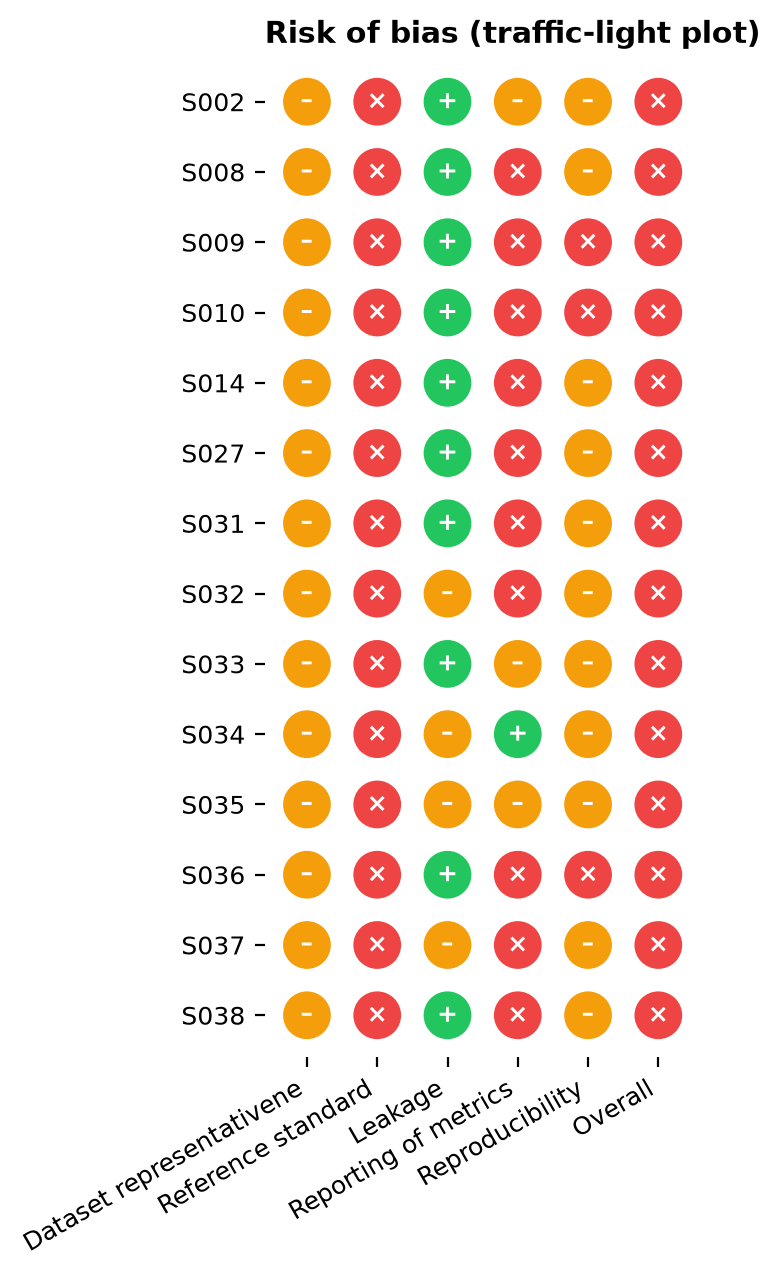
\includegraphics[width=0.5\linewidth]{risk_of_bias.png}
\caption{Risk of bias per study and domain (green: low; orange: some concerns; red: high)}\label{fig:rob}
\end{figure}

\subsection{Results of individual studies}
Table~\ref{tab:res} lists the quantitative results, and Figure~\ref{fig:ss} plots sensitivity
and specificity.

\begin{table}[!htb]
\small
\setlength{\tabcolsep}{4pt}
\renewcommand{\arraystretch}{1.08}
\centering
\captionof{table}{Reported accuracy and efficiency of LLM screening}\label{tab:res}
\begin{tabular}{|p{2.7cm}|p{2.5cm}|p{2.5cm}|p{5.2cm}|}
\hline
Study & Sensitivity & Specificity & Other results\\
\hline
Li~\cite{s002} & 0.77 (recall) & -- & precision 0.34; NPV 1.00; DeepSeek-R1 F1 0.93, accuracy 0.88 on other topics\\
\hline
Fazeli~\cite{s008} & 0.832 & 0.852 & accuracy 0.851; PPV 0.198; NPV 0.991; 1,000 abstracts in 40 min vs 16 h\\
\hline
Dai~\cite{s027} & 0.73 (0.57--0.85) & 0.99 (0.97--0.99) & pooled; AUC 0.97; better than ASReview, Abstrackr\\
\hline
Cao~\cite{s031} & 0.967 & 0.979 & humans 0.817 / 0.981 on the same task\\
\hline
Homiar~\cite{s032} & 1.00$^a$ & moderate & simulated workload reduction 65--85\%\\
\hline
Cao~\cite{s033} & 0.977 (0.867--1.0) & 0.852 (0.683--0.959) & zero-shot sensitivity 0.49; $<$1 day, US\$157 vs $>$83 h, US\$1,667\\
\hline
Vallamchetla~\cite{s034} & 1.00$^b$ & 0.999$^b$ & $\kappa$ 0.998; screening time cut by about 75\%\\
\hline
Dogra~\cite{s035} & variable & high & F1 0.389--0.854; authority bias towards human labels\\
\hline
Han~\cite{s036} & $>$0.925$^c$ & -- & CoT few-shot best precision--recall balance\\
\hline
Vivekanantha~\cite{s038} & 0.941--1.00 & $>$0.923 & all metrics $>$0.923; 6.5--17.4 abstracts/min\\
\hline
Laignelot~\cite{s014} & 0.92 (0.69--0.98)$^d$ & 0.89 (0.72--0.95)$^d$ & median positive/negative percent agreement, 63 studies\\
\hline
Kim~\cite{s037} & 1.00$^e$ & 0.81$^e$ & SROC sensitivity and specificity near 0.90; 1.7 s per entry\\
\hline
\multicolumn{4}{|p{13.6cm}|}{\footnotesize $^a$ for studies included after full text; $^b$ humans assisted by LLM-generated PICOS summaries; $^c$ GPT-4o and DeepSeek; $^d$ median (IQR); $^e$ the authors' new tool. Hida~\cite{s009} and Mosaed~\cite{s010} reported variability and domain effects without a single pooled value.}\\
\hline
\end{tabular}
\end{table}

\begin{figure}[!htb]
\centering
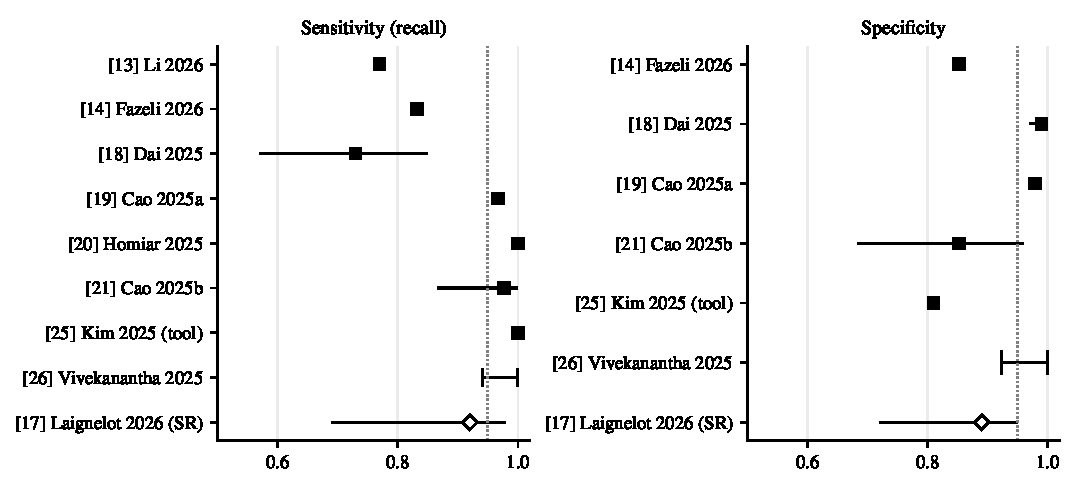
\includegraphics[width=0.96\linewidth]{sens_spec.pdf}
\caption{Reported sensitivity and specificity of LLM screening (bars: CI, range or IQR, shown without a point when only a range was reported; open diamonds: prior systematic review; dotted line: 0.95, a common target for screening sensitivity)}\label{fig:ss}
\end{figure}

\subsection{Results of syntheses}
\textbf{Theme 1: accuracy.} \emph{Low certainty.} Sensitivity was high in most primary studies:
0.94 to 1.00 for GPT-5~\cite{s038}, 0.967 for a GPT-4.1 agent that outperformed dual human
review on the same task (human 0.817)~\cite{s031}, 0.977 for optimised GPT-4
prompts~\cite{s033} and 1.00 for refined GPT-4o prompts~\cite{s032}. The lowest values came from a
single cost-efficient model (GPT-4o mini, 0.832~\cite{s008}), a hybrid pipeline optimised for
a different trade-off (recall 0.77~\cite{s002}), and a pooled estimate across six thoracic
meta-analyses (0.73~\cite{s027}). Specificity was more heterogeneous, from 0.81~\cite{s037} to
0.99~\cite{s027}. The prior reviews agree: median agreement with humans was 0.92 for
inclusions and 0.89 for exclusions across 63 studies~\cite{s014}.

\textbf{Theme 2: efficiency.} \emph{Low certainty.} Every study that measured time or cost
found large savings. Examples are 1,000 abstracts in 40 minutes instead of 16 hours~\cite{s008},
under one day and US\$157 instead of more than 83 hours and US\$1,667~\cite{s033}, 6.5 to 17.4
abstracts per minute~\cite{s038}, and simulated workload reductions of 65--85\%~\cite{s032}. As
an assistant rather than a replacement, LLM-generated PICOS summaries cut human screening time
by about 75\% while improving sensitivity~\cite{s034}. These estimates seldom include the time
needed for human quality control~\cite{s008}.

\textbf{Theme 3: variability.} \emph{Low certainty.} Performance depended on the prompt, the
model, the domain and even the run. Zero-shot prompts reached only 0.49 sensitivity where
optimised templates reached 0.977~\cite{s033}. Chain-of-thought few-shot prompting gave the
best precision--recall balance~\cite{s036}. Recall was high in broad clinical tasks but poor in
a narrowly scoped preclinical task until a pre-specified prompt revision~\cite{s010}. Repeated
runs of the same model on the same records produced different decisions~\cite{s009}, so
non-determinism must be reported and controlled.

\textbf{Theme 4: agreement and human oversight.} \emph{Low certainty.} Agreement was very high
when LLMs assisted humans ($\kappa=0.998$~\cite{s034}). Models confronted with a disagreement
tended to defer to the label presented as human, a form of authority bias~\cite{s035}. Several
authors therefore recommend a human-in-the-loop, sensitivity-first use: the LLM excludes
confidently irrelevant records and humans verify the rest~\cite{s010,s035,s037}.

\subsection{Certainty of evidence}
Certainty was rated low for all four themes. It was downgraded for risk of bias (imperfect
reference standards), inconsistency (heterogeneous metrics and domains) and imprecision
(few confidence intervals). Reporting bias cannot be excluded: positive evaluations are more
likely to be published, and half of the evidence comes from preprints.

% =============================================================================
\section{Discussion}
\textbf{Summary.} Current LLMs screen titles and abstracts with high sensitivity, often above
the 0.95 commonly required for a first screener, and at a small fraction of the time and cost
of human reviewers. Their specificity is lower and more variable, so many irrelevant records
still need to be read. The best results combine a strong model, an optimised prompt and a
sensitivity-first policy. In one study an LLM agent was more sensitive than dual human review
on the same records~\cite{s031}.

\textbf{Implications.} The evidence supports using LLMs as a first or second screener under
human supervision, not as an autonomous replacement. In practice, reviewers should:
\begin{enumerate}[label=(\arabic*),leftmargin=2.2em,itemsep=2pt,topsep=2pt,parsep=0pt]
\item pre-specify the prompt and freeze the model version;
\item validate sensitivity on a calibration sample from their own review;
\item repeat the runs or fix the sampling to control non-determinism;
\item report the screening process transparently.
\end{enumerate}
The pipeline used for this review follows these recommendations: dual independent agents,
adjudication by a different model family, human checkpoints, and an audit trail of every
decision.

\textbf{Limitations of the evidence.} The included studies relied on human decisions as an
imperfect reference standard, used convenience samples of completed reviews, rarely addressed
pre-training leakage, and reported heterogeneous metrics, which prevented a meta-analysis.

\textbf{Limitations of this review.} The screening, extraction and appraisal were carried out
by local open-weight LLM agents rather than two human reviewers. Their decisions are fully
traceable, but they were not all verified by a human. The search used the first 25 records per
query of three databases (Semantic Scholar was rate-limited). A full-text budget left 26
potentially eligible records unassessed, and 9 of the 15 assessed reports were read on the
abstract only. The risk-of-bias tool was adapted rather than validated. The review therefore
probably under-represents the literature, and its findings should be read as a rigorous,
reproducible rapid review.

% =============================================================================
\section{Conclusions}
Across 14 recent studies, LLMs achieved sensitivity between 0.73 and 1.00 and specificity
between 0.81 and 0.99 for title and abstract screening, while reducing workload by roughly
two thirds to three quarters and cutting time from days to hours. The certainty of this evidence
is low, because of imperfect reference standards and heterogeneous reporting. LLMs are
therefore ready to accelerate screening under human oversight, and they should be evaluated
with standardised metrics, frozen model versions and reproducible protocols. Future work should
benchmark LLM screeners against adjudicated gold standards across many reviews, and report
non-determinism and cost alongside accuracy.

\textbf{Declarations.} \emph{AI use:} this review was produced with PRISMA-Agent, a
multi-agent pipeline (LangGraph; local models \texttt{qwen3:8b}, \texttt{gpt-oss:20b},
\texttt{nomic-embed-text}). The protocol, search log, screening decisions with rationales,
extraction with verified quotations, full audit trail and reproducibility manifest are
available in~\cite{repo}. \emph{Funding:} none. \emph{Competing interests:} none.

% =============================================================================
\begin{thebibliography}{99}

\bibitem{prisma} M. J. Page et al., The PRISMA 2020 statement: An updated guideline for
reporting systematic reviews, \textit{BMJ}, vol.372, n71, 2021.

\bibitem{borah} R. Borah, A. W. Brown, P. L. Capers and K. A. Kaiser, Analysis of the time and
workers needed to conduct systematic reviews of medical interventions using data from the
PROSPERO registry, \textit{BMJ Open}, vol.7, no.2, e012545, 2017.

\bibitem{cochrane} J. P. T. Higgins et al. (eds.), \textit{Cochrane Handbook for Systematic
Reviews of Interventions}, 2nd Edition, Wiley, Chichester, 2019.

\bibitem{cohen} J. Cohen, A coefficient of agreement for nominal scales, \textit{Educational
and Psychological Measurement}, vol.20, no.1, pp.37-46, 1960.

\bibitem{grade} G. H. Guyatt et al., GRADE: An emerging consensus on rating quality of evidence
and strength of recommendations, \textit{BMJ}, vol.336, no.7650, pp.924-926, 2008.

\bibitem{quadas} P. F. Whiting et al., QUADAS-2: A revised tool for the quality assessment of
diagnostic accuracy studies, \textit{Ann. Intern. Med.}, vol.155, no.8, pp.529-536, 2011.

\bibitem{rrf} G. V. Cormack, C. L. A. Clarke and S. Buettcher, Reciprocal rank fusion
outperforms Condorcet and individual rank learning methods, \textit{Proc. ACM SIGIR},
pp.758-759, 2009.

\bibitem{rag} P. Lewis et al., Retrieval-augmented generation for knowledge-intensive NLP
tasks, \textit{Proc. NeurIPS}, vol.33, pp.9459-9474, 2020.

\bibitem{mchugh} M. L. McHugh, Interrater reliability: The kappa statistic, \textit{Biochem.
Med.}, vol.22, no.3, pp.276-282, 2012.

\bibitem{landis} J. R. Landis and G. G. Koch, The measurement of observer agreement for
categorical data, \textit{Biometrics}, vol.33, no.1, pp.159-174, 1977.

\bibitem{repo} M. Haddad, \textit{PRISMA-Agent: An Agentic AI Pipeline for Systematic Reviews},
source code and review artefacts, https://github.com/HADDADmed/M1\_final\_project, 2026.

\bibitem{langgraph} LangChain, \textit{LangGraph Documentation},
https://langchain-ai.github.io/langgraph/, accessed November 2026.

\bibitem{s002} Y. Li, X. Du, Y. Wang et al., AI-assisted literature screening: A hybrid approach
using large language models and retrieval-augmented generation, \textit{Int. J. Med. Inform.},
2026, doi:10.1016/j.ijmedinf.2025.106205.

\bibitem{s008} M. S. Fazeli, E. Kasireddy, M.-M. Pourrahmat et al., Automating screening of titles
and abstracts in systematic reviews: An assessment of GPT-4o mini, \textit{medRxiv}, 2026,
doi:10.64898/2026.05.15.26353334.

\bibitem{s009} G. S. Hida, D. M. Ribeiro and E. Yahata, Beyond accuracy: LLM variability in evidence
screening for software engineering SLRs, \textit{arXiv}, 2026, doi:10.48550/arXiv.2604.27006.

\bibitem{s010} R. Mosaed, A. Ziaee, A. Salehi-Abargouei and M. Salehi-Marzijarani, Evaluation of a
prompt-standardized LLM pipeline for title--abstract screening: Cross-domain performance and
error taxonomy, \textit{OSF Preprints}, 2026.

\bibitem{s014} F. Laignelot, G. L. Martin, M. Ossman et al., Large language models show promising
performance for some systematic review tasks but call for cautious implementation: A systematic
review, \textit{J. Clin. Epidemiol.}, 2026, doi:10.1016/j.jclinepi.2026.112221.

\bibitem{s027} Z.-Y. Dai, F.-Q. Wang, C. Shen et al., Accuracy of large language models for
literature screening in thoracic surgery: Diagnostic study, \textit{J. Med. Internet Res.}, 2025,
doi:10.2196/67488.

\bibitem{s031} C. Cao, R. Arora, P. Cento et al., Automation of systematic reviews with large
language models, \textit{medRxiv}, 2025, doi:10.1101/2025.06.13.25329541.

\bibitem{s032} A. Homiar, J. Thomas, E. G. Ostinelli et al., Development and evaluation of prompts
for a large language model to screen titles and abstracts in a living systematic review,
\textit{BMJ Ment. Health}, 2025, doi:10.1136/bmjment-2025-301762.

\bibitem{s033} C. Cao, J. Sang, R. Arora et al., Development of prompt templates for large language
model-driven screening in systematic reviews, \textit{Ann. Intern. Med.}, 2025,
doi:10.7326/ANNALS-24-02189.

\bibitem{s034} S. K. Vallamchetla, O. Abdelkader, A. Elnaggar et al., Do it faster with PICOS:
Generative AI-assisted systematic review screening, \textit{J. Biomed. Inform.}, 2025,
doi:10.1016/j.jbi.2025.104860.

\bibitem{s035} S. Dogra, S. Arabshahi, J. Wei et al., Evaluating large language models for
radiology systematic review title and abstract screening, \textit{Acad. Radiol.}, 2025,
doi:10.1016/j.acra.2025.08.014.

\bibitem{s036} B. Han, A. Mathrani and T. Susnjak, Evaluating prompting strategies and large
language models in systematic literature review screening: Relevance and task-stage
classification, \textit{arXiv:2510.16091}, 2025.

\bibitem{s037} J. K. Kim, M. Rickard, P. Dangle et al., Evaluating large language models for
title/abstract screening: A systematic review and meta-analysis \& development of new tool,
\textit{J. Med. Artif. Intell.}, 2025, doi:10.21037/jmai-24-408.

\bibitem{s038} P. Vivekanantha, H. Son, L. Bernardini et al., Evaluating the efficacy and
efficiency of GPT-5 for automated title and abstract screening in orthopedic surgery systematic
reviews, \textit{Curr. Rev. Musculoskelet. Med.}, 2025, doi:10.1007/s12178-025-10001-y.

\end{thebibliography}

\end{document}
